\documentclass{article}
\usepackage[margin=0.75in]{geometry}
\usepackage{xcolor}
\usepackage{amsmath}
\usepackage{amssymb}
\usepackage{fontspec}
\usepackage{tikz}
\usetikzlibrary{tikzmark, arrows.meta, positioning, decorations.pathreplacing}
\usepackage{enumitem}
\usepackage{multicol}

% ---- Theme Colors ----
\definecolor{bglight}{HTML}{FFFFFF}
\definecolor{textlight}{HTML}{000000}
\definecolor{subtext}{HTML}{666666}

% ---- Bar Model Visual Colors ----
\colorlet{redbar}{red!70!black}
\colorlet{bluebar}{blue!55!black}
\colorlet{arrowblue}{cyan!70!blue}

\pagecolor{bglight}
\color{textlight}

\pagestyle{empty}

% Numbered node macro from your theme
\newcommand{\stepnum}[2]{%
  \tikzmarknode{#2}{%
    \begin{tikzpicture}[baseline=(char.base)]
      \node[draw=textlight, circle, inner sep=1.5pt, font=\sffamily\small] (char) {#1};
    \end{tikzpicture}%
  }%
}

\begin{document}
\sffamily

% ================= HEADER =================
\begin{center}
  {\Huge \bfseries Bar Method Exercise Sheet} \\[0.4em]
\end{center}
\vspace{1em}

\section*{Part 1: Visualizing Addition}

% ================= EXAMPLE SECTION =================
{\Large \textbf{Example: Finding Total Pencils}}
\vspace{0.3em}

\noindent Maya has \textbf{5 red pencils} and \textbf{3 blue pencils}. How many pencils does she have in total?
\vspace{0.8em}

\begin{description}[leftmargin=2em]

  \item[\stepnum{1}{s1}] \textbf{Identify and label the parts}\\[0.2em]
  Determine the quantities given in the problem:
  \begin{itemize}
    \item Red pencils = $5$
    \item Blue pencils = $3$
  \end{itemize}
  \vspace{0.6em}

  \item[\stepnum{2}{s2}] \textbf{Draw bars representing each part}\\[0.4em]
  Draw connected blocks proportional to each value to visualize the whole:
  \\[0.6em]
  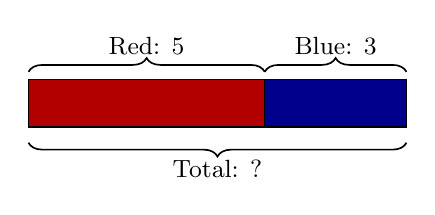
\begin{tikzpicture}[>=Stealth, baseline={(0,1.2)}]
    % Top brackets with labels
    \draw[decorate, decoration={brace, amplitude=5pt}, line width=0.6pt] (0, 1.8) -- (3, 1.8);
    \node[anchor=south] at (1.5, 1.9) {\small Red: 5};

    \draw[decorate, decoration={brace, amplitude=5pt}, line width=0.6pt] (3, 1.8) -- (4.8, 1.8);
    \node[anchor=south] at (3.9, 1.9) {\small Blue: 3};

    % Bars
    \draw[fill=redbar, draw=black, line width=0.5pt] (0, 1.1) rectangle (3, 1.7);
    \draw[fill=bluebar, draw=black, line width=0.5pt] (3, 1.1) rectangle (4.8, 1.7);

    % Bottom bracket for total
    \draw[decorate, decoration={brace, amplitude=5pt, mirror}, line width=0.6pt] (0, 0.9) -- (4.8, 0.9);
    \node[anchor=north] at (2.4, 0.8) {\small Total: ?};
  \end{tikzpicture}
  \vspace{0.6em}

  \item[\stepnum{3}{s3}] \textbf{Write and solve the equation}\\[0.4em]
  Combine the parts to calculate the overall total:
  \[
    5 + 3 = \mathbf{8} \quad \text{or} \quad 3 + 5 = \mathbf{8}
  \]
  \vspace{0.2em}
  Maya has \textbf{8 pencils} altogether.

\end{description}

\begin{tikzpicture}[remember picture, overlay]
  \draw[dotted, thick, textlight!60] (s1.south) -- (s2.north);
  \draw[dotted, thick, textlight!60] (s2.south) -- (s3.north);
\end{tikzpicture}

\vspace{1em}
\noindent\textcolor{subtext!40}{\rule{\linewidth}{0.5pt}}
\vspace{1.5em}

% ================= PRACTICE QUESTIONS =================
\begingroup
\parindent=0pt

{\Large \textbf{Practice Questions}}\par\vspace{0.4em}
Read each problem, fill in the missing numbers in the bar model, and write the final addition equation.

\endgroup
\vspace{1.5em}

\begin{enumerate}[label=\textbf{\arabic*.}, itemsep=2.5em, leftmargin=2em]

  % Question 1
  \item \textbf{Liam baked 6 chocolate cookies and 4 vanilla cookies. How many cookies did he bake in total?}

  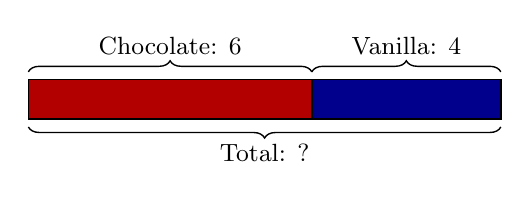
\begin{tikzpicture}[>=Stealth, baseline={(0,0.5)}]
    % Top brackets & Labels
    \draw[decorate, decoration={brace, amplitude=4pt}, line width=0.5pt] (0, 1.2) -- (3.6, 1.2);
    \node[anchor=south] at (1.8, 1.3) {\small Chocolate: 6};

    \draw[decorate, decoration={brace, amplitude=4pt}, line width=0.5pt] (3.6, 1.2) -- (6.0, 1.2);
    \node[anchor=south] at (4.8, 1.3) {\small Vanilla: 4};

    % Colored Bars
    \draw[fill=redbar, draw=black, line width=0.5pt] (0, 0.6) rectangle (3.6, 1.1);
    \draw[fill=bluebar, draw=black, line width=0.5pt] (3.6, 0.6) rectangle (6.0, 1.1);

    % Total Bracket
    \draw[decorate, decoration={brace, amplitude=4pt, mirror}, line width=0.5pt] (0, 0.5) -- (6.0, 0.5);
    \node[anchor=north] at (3.0, 0.4) {\small Total: ?};
  \end{tikzpicture}

  \vspace{0.5em}
  Equation: $\underline{\hspace{1.5cm}} + \underline{\hspace{1.5cm}} = \underline{\hspace{1.5cm}}$
  \hspace{2cm} Total cookies = $\underline{\hspace{1.5cm}}$

\end{enumerate}

\end{document}